\documentclass{article}

\usepackage{arxiv}
\usepackage[utf8]{inputenc}
\usepackage[T1]{fontenc}
\usepackage{hyperref}
\usepackage{url}
\usepackage{booktabs}
\usepackage{amsfonts,amsmath,amssymb}
\usepackage{mathrsfs}
\usepackage{microtype}
\usepackage{graphicx}
\usepackage{float}
\usepackage{caption}
\usepackage{subcaption}
\usepackage{xcolor}
\graphicspath{{figures/}{../figures/}}
\hypersetup{colorlinks=true,linkcolor=black,citecolor=blue,urlcolor=blue}
\captionsetup{font=small,labelfont=bf}
\setlength{\textfloatsep}{8pt plus 2pt minus 2pt}
\setlength{\floatsep}{6pt plus 2pt minus 2pt}
\setlength{\abovecaptionskip}{3pt}
\renewcommand{\topfraction}{0.9}
\renewcommand{\textfraction}{0.08}
\renewcommand{\floatpagefraction}{0.85}
\setcounter{topnumber}{3}\setcounter{totalnumber}{5}

\floatstyle{ruled}
\newfloat{algorithm}{tbp}{loa}
\floatname{algorithm}{Algorithm}

\newcommand{\A}{\mathscr{A}}
\newcommand{\D}{\mathscr{D}}
\newcommand{\R}{\mathscr{R}}
\newcommand{\T}{\mathscr{T}}
\newcommand{\Tres}{\mathscr{T}_{\mathrm{res}}}

\renewcommand{\shorttitle}{Decentralised Multi-Agent Search and Rescue}

\title{Decentralised Multi-Agent Search and Rescue under Limited Communication}

\author{
Boinapally Dhanvini\\
ID: 24110079\\
Branch: Artificial Intelligence\\
\texttt{boinapally.dhanvini@iitgn.ac.in}
\And
Bollineni Snehitha Rao\\
ID: 24110081\\
Branch: Artificial Intelligence\\
\texttt{snehitha.bollineni@iitgn.ac.in}
\And
Jils Shah\\
ID: 24110148\\
Branch: Computer Science\\
\texttt{jils.shah@iitgn.ac.in}
\AND
Thaker Shivangi Pareshkumar\\
ID: 24110371\\
Branch: Computer Science\\
\texttt{shivangi.thaker@iitgn.ac.in}
}

\begin{document}
\maketitle

\begin{abstract}
A person is trapped at an unknown location inside a hazardous building, and a team of heterogeneous
autonomous agents must locate them and bring them to an exit. Search drones sense well but cannot
perform the rescue; ground rescue robots can perform the rescue but sense poorly, so information
must travel from the agents that locate the victim to the agents that can reach them. Communication,
however, is a limited resource. We model the building as a graph with obstacles, hazards, an exit and one
hidden victim; the floor plan itself is unknown and discovered by sensing, agents keep Bayesian beliefs built from
noisy local scans, and they allocate tasks under a team communication budget $B$. A centralised baseline solves the
task-allocation CSP exactly with the Hungarian method on pooled information; the decentralised method solves the
corresponding DCOP with MGM or DSA-C over a range-limited communication graph. Over 30{,}600 simulated episodes we
find that (i) two messages per agent---the drone-to-robot handoff---recover 90\% of the success lost without
communication (success $0.66\!\to\!0.96$); (ii) with unrestricted budget the decentralised team succeeds in 99\% of
runs using 48\% of the centralised message volume, but is 21\% slower, half of that gap being due to having to discover
and share the map; (iii) communication is worth more when sensors are noisy, while intermediate budgets let partial,
noisy evidence spread and make robots chase false alarms; and (iv) coordination messages pay off only with a large
budget, where the cheaper DSA-C matches or beats MGM.
\end{abstract}

\keywords{Multi-agent systems \and Search and rescue \and Decentralised coordination \and Task allocation \and Constraint satisfaction \and Distributed constraint optimisation \and Limited communication}

\section{Introduction}
Search-and-rescue operations in hazardous buildings are difficult because responders often do not know where a trapped
person is, or which routes remain safe. Autonomous robots can support such operations by exploring, sensing and
mapping, and multi-robot teams have been studied extensively for exactly this setting~\cite{queralta2020}. Teams that mix
robots with different capabilities have also been studied for urban search and rescue, where the question of which robot
should take which task becomes central~\cite{gunn2015}.

This project considers a team of heterogeneous agents inside a simulated hazardous building: \emph{search drones}, which
move quickly and sense over a wide area but cannot rescue anyone, and \emph{ground rescue robots}, which move only along
accessible ground routes and sense poorly but can carry the victim to an exit. The split is deliberate: the agents that
find the victim are never the agents that can rescue the victim, so a report has to travel from one group to the other.
Three properties make this a multi-agent problem rather than a path-planning one: no agent observes the whole
environment; capabilities are complementary, so tasks must be allocated to agents able to perform them~\cite{korsah2013};
and communication is limited, so agents must decide not only where to go but also what is worth saying. Such coordination
is naturally modelled as a distributed constraint optimisation problem (DCOP)~\cite{fioretto2018}.

\textbf{Research question.} \emph{How does reducing the communication budget affect decentralised coordination in
multi-agent search and rescue when agents have incomplete and noisy information?} Secondary questions are whether
communication becomes more or less valuable as sensors become less reliable, how far decentralised coordination stays
from a centralised coordinator with pooled information, and how much redundant exploration~\cite{burgard2005} appears when
agents cannot talk. This report completes the project review with the methodology (Section~\ref{sec:method}), the
results (Section~\ref{sec:results}) and the individual contributions (Section~\ref{sec:contrib}).

\section{Preliminaries}
\textbf{Agents and heterogeneity.} $\A=\D\cup\R$, $\D\cap\R=\emptyset$, where $\D$ are search drones and $\R$ ground
robots. Drones have a larger sensing radius and higher reliability; only robots can rescue.
\textbf{Environment.} The building is a graph $G=(V,E)$ generated as a 2D grid whose cells are free, obstacles or
hazardous, with one exit $v_{\mathrm{exit}}$ and one victim location $v^\star$ unknown to the agents; time is discrete.
\textbf{Incomplete information.} A \emph{local observation} is what an agent's sensors return at its location; it is
\emph{noisy}: a scan may miss the victim or report one where there is none.
\textbf{Tasks.} $\T$ is the set of candidate tasks (searching a region, carrying out the rescue) with rescue tasks
$\Tres\subset\T$; \emph{task allocation} assigns tasks to capable agents~\cite{korsah2013}.
\textbf{Communication.} Agents exchange short messages; the total they may send in a run is limited by a budget $B$.
\textbf{CSP and DCOP.} A CSP is a triple of variables, domains and constraints; a DCOP distributes the variables among
agents and replaces constraints by cost functions that agents minimise by exchanging messages with
neighbours~\cite{fioretto2018}.

\section{Problem Formulation}\label{sec:formulation}
Let $p_i^t\in V$ be the location of agent $i$ at time $t$. \textbf{Decision variables:} $x_{ij}=1$ if task $j\in\T$ is
assigned to agent $i\in\A$ and $0$ otherwise. \textbf{Assignment constraints:}
\begin{align}
&\textstyle\sum_{i\in\A}x_{ij}\le 1 \;\;\forall j\in\T, \label{eq:c2}\\
&x_{ij}\le F_{ij}\;\;\forall i,j, \qquad F_{ij}=0\;\;\forall i\in\D,\ j\in\Tres, \label{eq:c4}
\end{align}
where $F_{ij}\in\{0,1\}$ is agent $i$'s capability for task $j$. \textbf{Observation model.} A scan by agent $i$ returns,
for every $v$ within radius $\rho_i$, a reading $z_v\in\{0,1\}$ with
\begin{equation}
\Pr(z_v=1\mid v=v^\star)=p^{\mathrm{det}}_i,\qquad \Pr(z_v=1\mid v\neq v^\star)=p^{\mathrm{fa}}_i,\label{eq:obs}
\end{equation}
with $p^{\mathrm{det}}_i>p^{\mathrm{det}}_{i'}$ and $\rho_i>\rho_{i'}$ for $i\in\D$, $i'\in\R$.
\textbf{Communication constraint.} $C_{\mathrm{comm}}=\sum_{t=1}^{T}\sum_{i\in\A}c(m_i^t)\le B$.
\textbf{Objective.} With completion time $T_{\mathrm{rescue}}$, movement cost $C_{\mathrm{move}}$ and success $S\in\{0,1\}$
($T_{\mathrm{rescue}}$ is set to the step limit when $S=0$),
\begin{equation}
\min_{\{x_{ij}\}}\; J=\lambda_tT_{\mathrm{rescue}}+\lambda_cC_{\mathrm{comm}}+\lambda_mC_{\mathrm{move}}+\lambda_f(1-S)
\quad\text{s.t. \eqref{eq:c2}--\eqref{eq:c4} and } C_{\mathrm{comm}}\le B.\label{eq:obj}
\end{equation}
\textbf{Decentralised form.} The DCOP $\langle\A,X,D,F,\alpha\rangle$ has variables $X=\{x_{ij}\}$, domains $\{0,1\}$, cost
functions $F$ derived from~\eqref{eq:obj} and $\alpha(x_{ij})=i$; each agent chooses its own variables from local
observations and received messages. The centralised problem is the same optimisation with all variables controlled
by one coordinator and $C_{\mathrm{comm}}$ not charged.

\section{Methodology}\label{sec:method}
Everything below is implemented in Python (NumPy/SciPy) in the accompanying repository; module names are given in
\texttt{typewriter}. Both approaches run on the \emph{same} simulator and the \emph{same} randomly generated building
for a given seed, and share the cost functions, so the only differences are who holds which information and how the
allocation is solved.

\subsection{Simulator (\texttt{sar/env.py}, \texttt{sar/agent.py}, \texttt{sar/mapknow.py})}
\textbf{Building.} An $n\times n$ grid ($n=20$ by default) receives a few internal walls with door gaps (room
structure), random debris obstacles (density 0.08) and hazard cells (density 0.06). The exit lies on the left wall; the
victim is placed uniformly among robot-reachable cells at least $0.6n$ steps from the exit. Drones fly over hazards but
not through walls; robots may not enter hazards. All agents enter at the exit (drones 2 cells/step, robots 1
cell/step).
\textbf{Unknown floor plan.} As in the review, the state of unvisited locations is unknown: each agent holds its own
terrain map in which every cell is \emph{unknown} until it falls inside the agent's sensing window (or a teammate reports
it). Agents plan shortest paths on this map \emph{optimistically}---unknown cells are assumed traversable for their
movement model---and re-plan every step; an agent that runs into an undiscovered wall or hazard learns it and re-routes.
Cells revealed to be obstacles or hazards are removed from the victim posterior. A \emph{known-map} variant (the floor
plan given from blueprints) is kept for comparison (E6).
\textbf{Sensing and belief.} Drones scan a $5\times5$ window ($\rho=2$), robots a $3\times3$ window ($\rho=1$), with the
reliability presets of Table~\ref{tab:params}. Each agent keeps a posterior $b_i(v)=\Pr(v^\star=v\mid\text{evidence})$,
initially uniform over all cells (over robot-reachable cells when the map is known). Since there is a single victim, a reading $z_v$ from a sensor with
parameters $(p^{\mathrm{det}},p^{\mathrm{fa}})$ multiplies $b(v)$ by the likelihood ratio
\begin{equation}
L(z_v)=\Big(\tfrac{p^{\mathrm{det}}}{p^{\mathrm{fa}}}\Big)^{z_v}\Big(\tfrac{1-p^{\mathrm{det}}}{1-p^{\mathrm{fa}}}\Big)^{1-z_v}
\label{eq:bayes}
\end{equation}
followed by renormalisation (all other cells share the same denominator). Updates are kept in log space. A robot that
stands on a cell physically checks it: if the victim is there it picks them up, otherwise the cell's posterior is set
to zero (certain absence). An agent \emph{claims} the victim at $\hat v=\arg\max_v b_i(v)$ when $b_i(\hat v)\ge\tau=0.7$.

\subsection{Communication model and messaging rule (\texttt{sar/sim.py})}
A message is a broadcast received by every agent within Euclidean range $r_c=9$ cells; each costs one unit
($c(m)=1$). The team budget is split equally, each agent holding a quota $\lfloor B/|\A|\rfloor$, so
$C_{\mathrm{comm}}\le B$ holds by construction and needs no global counter. Neighbour discovery (who is in range) is free.
As promised in the review, \emph{what} to send is fixed to one simple rule so that the budget remains the variable
under study. Each agent buffers its unshared scans; an \texttt{OBS} message carries the whole buffer (so receivers apply
exactly the update~\eqref{eq:bayes} with the sender's sensor parameters), the terrain it has discovered, the sender's
current task, its cleared cells and its current claim. Messages are sent in priority order: (1)~\emph{urgent}: a new or retracted claim, a robot's
report that a claimed cell was empty, or the ``victim picked up'' notice; (2)~\emph{delivery}: a drone holding its own
claim that has not yet reached a robot flies towards the last known robot position and broadcasts once a robot is in
range; (3)~\emph{relay}: a newly heard claim is re-broadcast once; (4)~\emph{periodic}: every 5 steps the observation
buffer is shared; (5)~DCOP messages (Section~\ref{sec:mgm}). Classes (4)--(5) are only sent while an agent has more
than a reserve of 2 messages left, so the reserve is kept for victim reports.
\textbf{Conflicting reports.} Each agent keeps the latest claim per sender and its own claim; it acts on the one with the
highest confidence (ties: most recent), and discards claims on cells it knows to be empty.

\subsection{Task set and cost functions (\texttt{sar/allocation.py})}
The map is split into $K=16$ regions ($4\times4$). The task set is $\T=\{\textsc{search}_k\}_{k=1}^{K}\cup\{\textsc{rescue}\}\cup\{\textsc{idle}\}$,
where \textsc{idle} plays the role of ``unassigned'' and is exempt from~\eqref{eq:c2}. For agent $i$ with belief $b_i$,
speed $s_i$ and distance $d_i(\cdot)$ in its own movement graph, the unary costs instantiate the time and failure terms
of~\eqref{eq:obj}:
\begin{equation}
u_i(\textsc{search}_k)=\frac{d_i(k)}{s_i}-w_{\mathrm{info}}\,q_i\!\!\sum_{v\in\text{region }k}\!\! b_i(v),\quad
u_i(\textsc{rescue})=\frac{d_i(\hat v)}{s_i}-w_{\mathrm{res}}\,b_i(\hat v),\quad u_i(\textsc{idle})=0,
\end{equation}
where $q_i=p^{\mathrm{det}}_i(2\rho_i+1)^2/25$ is the scanning efficiency and \textsc{rescue} exists only when the agent
holds a claim $\hat v$. $u_i(\textsc{rescue})=+\infty$ for drones encodes~\eqref{eq:c4}. The pairwise cost
$w(x_i,x_j)=w_{\mathrm{dup}}\,[x_i=x_j\neq\textsc{idle}]$ is the soft form of~\eqref{eq:c2}. Given its task, an agent moves
to the cell of its region maximising (posterior mass in its sensing window)$/(1+0.1\,d_i)$; a rescuer moves to $\hat v$
and, once carrying, to the exit; \textsc{idle} agents hold position (this is what drones do once the belief has
collapsed, saving movement).

\subsection{Centralised baseline: exact assignment}
A coordinator receives every scan every step (counted as one uplink message per agent per step, plus one downlink per
changed assignment, but never limited), maintains one pooled belief and terrain map, and every 5 steps (or when a
claim appears) solves
$\min\sum_i u_i(x_i)$ subject to~\eqref{eq:c2}--\eqref{eq:c4} \emph{exactly}: rows are agents, columns the non-idle tasks
plus one private \textsc{idle} column per agent, infeasible pairs get cost $10^6$, and the rectangular assignment is
solved by the Hungarian method~\cite{kuhn1955} (SciPy \texttt{linear\_sum\_assignment}). Its optimality is
checked against brute-force enumeration of all feasible assignments, and constraint~\eqref{eq:c2} is never violated
(both verified in \texttt{tests/test\_model.py}).

\subsection{Decentralised DCOP coordination: MGM and DSA-C}\label{sec:mgm}
The review left the DCOP solver open. We implement two local-search solvers, MGM~\cite{maheswaran2004} (default) and
DSA-C~\cite{zhang2005}, rather than ADOPT~\cite{modi2005}: ADOPT is complete but
needs a DFS tree and a number of messages exponential in the worst case, which cannot be stopped at an arbitrary budget,
whereas MGM is an anytime local search whose cost is linear in rounds, whose solution quality never decreases between
rounds, and which degrades gracefully when messages are dropped---the regime we study. Every 5 steps each agent runs
the rounds of Algorithm~\ref{alg:mgm} using \emph{its own} belief; tasks of neighbours are remembered in an
\emph{agent view} that expires after 15 steps. Between rounds, an agent hit by a new claim re-decides locally. With
$B=0$ no \texttt{VALUE}/\texttt{GAIN} message is ever sent and the algorithm reduces to independent greedy choices---the
no-communication ablation. \textbf{DSA-C} uses the same \texttt{VALUE} phase but no \texttt{GAIN} messages: in each
round every agent moves to its best response with probability $p=0.7$ if this strictly lowers its local cost, or keeps
it equal while its current value conflicts with a neighbour's. It is cheaper per round than MGM but not monotone.
Finally, a \textbf{no-coordination ablation} sends only \texttt{OBS} messages (tasks are learned from their piggyback)
and lets every agent take its best response, isolating the value of coordination messages from the value of shared
observations.

\begin{algorithm}[t]
\small
\caption{One MGM allocation epoch at agent $i$ (decentralised; all agents run it in parallel)}\label{alg:mgm}
\begin{tabbing}
xx\=xx\=xx\=\kill
\textbf{input:} belief $b_i$, claim $\hat v$ (if any), agent view $\mathcal V_i$, quota left $Q_i$\\
compute unary costs $u_i(\cdot)$ on own domain; if current $x_i$ infeasible: $x_i\leftarrow\arg\min_x[u_i(x)+\sum_{j\in\mathcal V_i}w(x,x_j)]$\\
\textbf{for} round $=1..3$ \textbf{do}\\
\> \textbf{if} $x_i$ changed or announcement is stale \textbf{and} $Q_i>$ reserve: broadcast \texttt{VALUE}$(x_i)$ \hfill (cost 1)\\
\> on receiving \texttt{VALUE}$(x_j)$: $\mathcal V_i[j]\leftarrow(x_j,t)$\\
\> $x_i^\ast\leftarrow\arg\min_x\big[u_i(x)+\sum_{j\in\mathcal V_i,\,\text{fresh}}w(x,x_j)\big]$;\ \ $g_i\leftarrow \mathrm{cost}(x_i)-\mathrm{cost}(x_i^\ast)$\\
\> \textbf{if} $g_i>0$ \textbf{and} $Q_i>$ reserve: broadcast \texttt{GAIN}$(g_i)$ \hfill (cost 1)\\
\> \textbf{if} $g_i>0$ and $(g_i,-i)>(g_j,-j)$ for every gain $g_j$ heard this round: $x_i\leftarrow x_i^\ast$\\
\> \textbf{if} no agent changed: \textbf{break}
\end{tabbing}
\end{algorithm}

\subsection{Experimental setup (\texttt{experiments/run\_experiments.py})}
Default parameters are listed in Table~\ref{tab:params}. Each configuration is run on the same 300 seeds (matched
building instances) for every method and budget; we report means with 95\% confidence intervals. The objective weights
are $\lambda_t=1$, $\lambda_c=0.1$, $\lambda_m=0.05$, $\lambda_f=300$ and the step limit (survival window) is 150.
Experiments: \textbf{(E1)} budget $B\in\{0,10,20,40,80,160,320,\infty\}$ for MGM, DSA-C and the no-coordination
ablation;
\textbf{(E2)} E1 at three sensor-reliability levels; \textbf{(E3)} team size
$(|\D|,|\R|)\in\{(2,1),(3,2),(5,3)\}$ and \textbf{(E4)} building complexity (simple $15^2$, medium $20^2$, complex $28^2$
with increasing obstacle/hazard density and walls), both at $B\in\{0,20,80,\infty\}$ (none/low/moderate/unrestricted);
\textbf{(E5)} communication range $r_c\in\{4,6,9,14,\infty\}$ at $B\in\{40,\infty\}$; \textbf{(E6)} known vs.\ unknown
floor plan at $B\in\{0,20,80,\infty\}$. In total 30{,}600 episodes; the whole study runs in about 13 minutes on a
10-core laptop. Besides the four metrics of the review we log the handoff
time (first step a robot holds a correct claim), the number of steps in which~\eqref{eq:c2} is violated, robot trips to
false claims, and \emph{redundancy}: the fraction of scanned cells scanned by two or more agents.

\begin{table}[t]
\centering\small
\caption{Default parameters. Reliability is $(p^{\mathrm{det}},p^{\mathrm{fa}})$ per scanned cell.}\label{tab:params}
\begin{tabular}{@{}ll@{\hspace{2.5em}}ll@{}}
\toprule
Grid / regions & $20\times20$ / $4\times4$ & Team & 3 drones + 2 robots \\
Speed (drone / robot) & 2 / 1 cells per step & Sensing radius (drone / robot) & 2 / 1 \\
High reliability & drone (0.95, 0.01), robot (0.70, 0.02) & Comm.\ range $r_c$ & 9 cells \\
Medium (default) & drone (0.80, 0.03), robot (0.55, 0.04) & Claim threshold $\tau$ & 0.7 \\
Low reliability & drone (0.60, 0.06), robot (0.45, 0.07) & Replan period / DCOP rounds & 5 steps / 3 \\
$w_{\mathrm{info}}, w_{\mathrm{res}}, w_{\mathrm{dup}}$ & 400, 1000, 1000 & Share period / reserve & 5 steps / 2 msgs \\
\bottomrule
\end{tabular}
\end{table}

\begin{figure}[t]
\centering
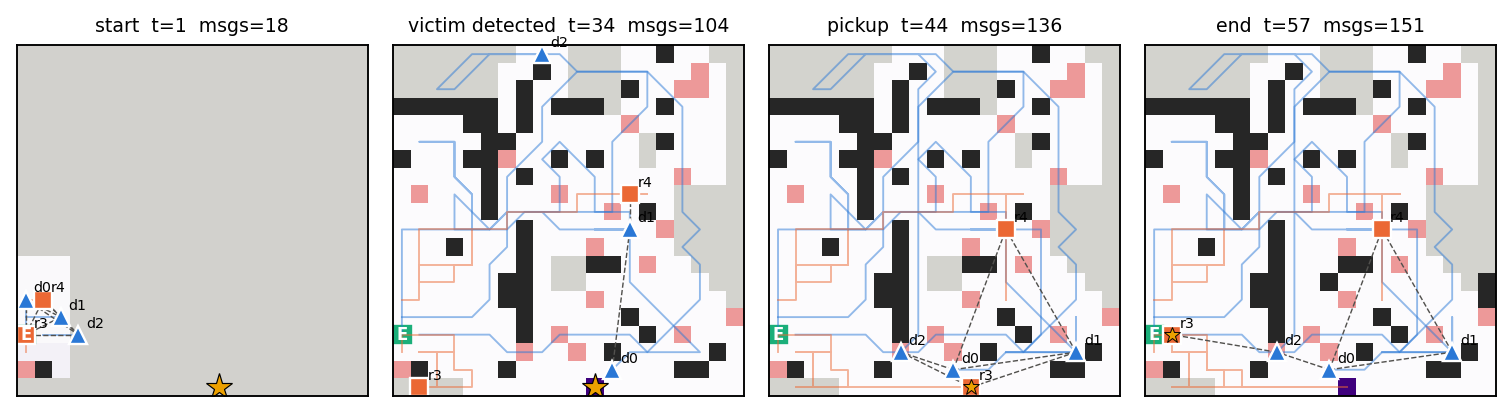
\includegraphics[width=\textwidth]{snapshots_dcop_Binf_s3.png}
\caption{A decentralised episode (seed 3, $B=\infty$) from the simulator: obstacles (black), hazards (red), exit (E),
drones $d_j$ (blue triangles), robots $r_j$ (orange squares), victim (star), communication links within range
(dashed), agent trajectories, drone $d_0$'s posterior (purple) and the cells $d_0$ has not discovered yet, directly or
through messages (grey). The victim is claimed at $t=34$, picked up by robot $r_3$ at $t=44$ and carried out at $t=57$.}
\label{fig:episode}
\end{figure}

\section{Results}\label{sec:results}

\begin{figure}[t]
\centering
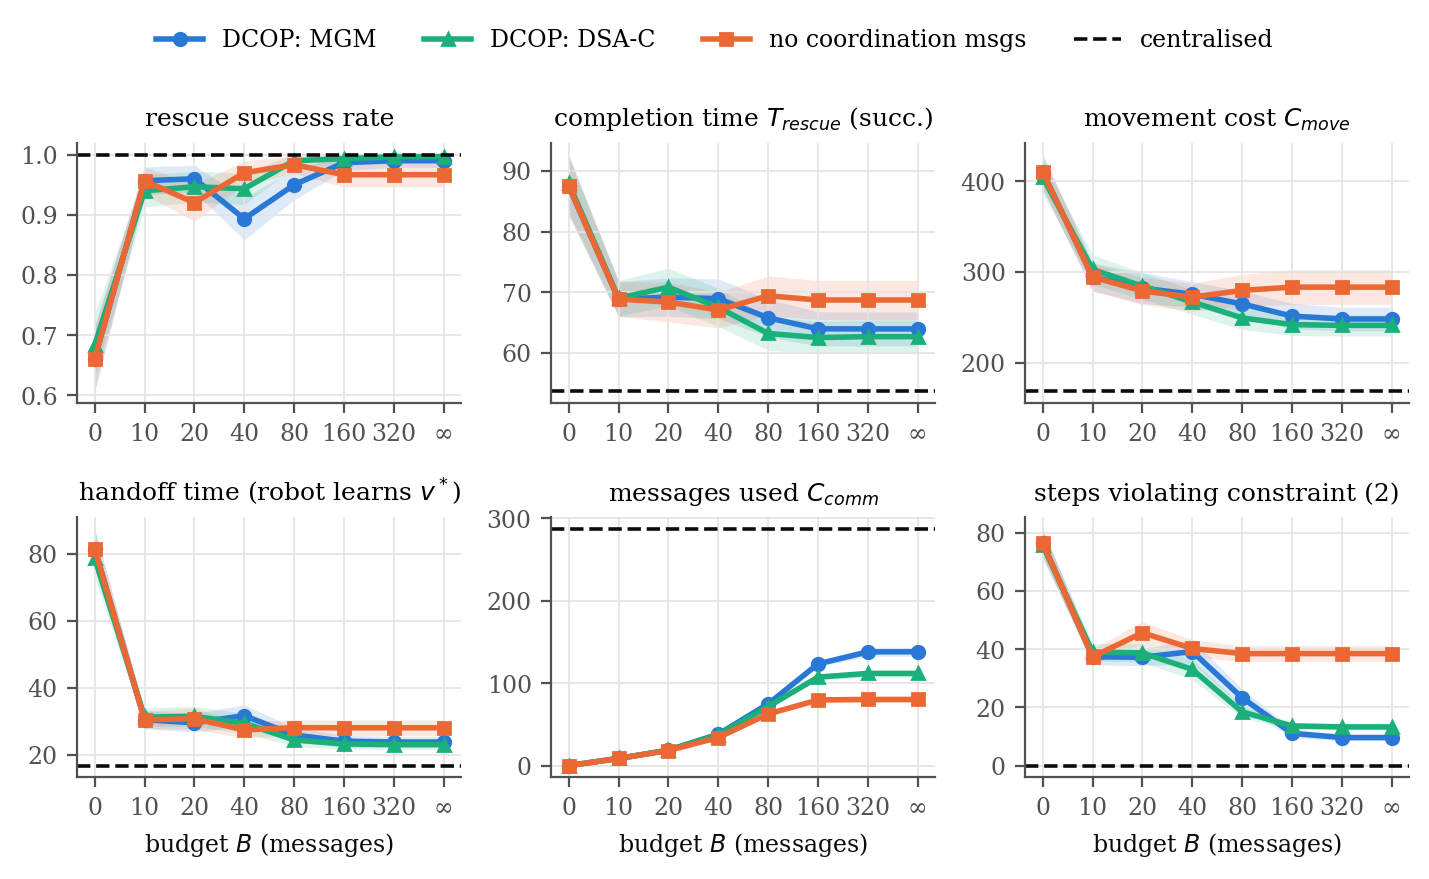
\includegraphics[width=\textwidth]{budget_main.png}
\caption{E1: metrics against the team budget $B$ (unknown map, medium reliability, 300 seeds; bands are 95\% CIs).
Dashed line: centralised reference. Completion time is averaged over successful runs.}
\label{fig:main}
\end{figure}

\begin{table}[t]
\centering\small
\caption{E1 summary (mean $\pm$ 95\% CI over 300 matched seeds). $T$ on successful runs; ``(2) viol.'' = steps in
which two agents hold the same non-idle task..}\label{tab:main}
\begin{tabular}{@{}llcccccc@{}}
\toprule
Method & $B$ & Success & $T_{\mathrm{rescue}}$ & $C_{\mathrm{comm}}$ & $C_{\mathrm{move}}$ & (2) viol. & Redund. \\
\midrule
Centralised & -- & 1.00\,$\pm$\,0.00 & 53.3\,$\pm$\,2.0 & 286.0\,$\pm$\,10.1 & 166\,$\pm$\,6 & 0.0 & 0.52 \\
\midrule
DCOP (MGM) & 0 & 0.74\,$\pm$\,0.05 & 85.5\,$\pm$\,4.4 & 0.0\,$\pm$\,0.0 & 364\,$\pm$\,18 & 77.5 & 0.81 \\
 & 10 & 0.89\,$\pm$\,0.03 & 68.2\,$\pm$\,3.3 & 9.0\,$\pm$\,0.2 & 288\,$\pm$\,17 & 48.4 & 0.78 \\
 & 20 & 0.92\,$\pm$\,0.03 & 67.4\,$\pm$\,3.2 & 18.8\,$\pm$\,0.2 & 280\,$\pm$\,16 & 44.8 & 0.78 \\
 & 40 & 0.94\,$\pm$\,0.03 & 67.0\,$\pm$\,3.3 & 38.2\,$\pm$\,0.2 & 265\,$\pm$\,15 & 37.9 & 0.71 \\
 & 80 & 0.98\,$\pm$\,0.02 & 60.4\,$\pm$\,2.8 & 74.1\,$\pm$\,0.5 & 240\,$\pm$\,13 & 20.0 & 0.68 \\
 & $\infty$ & 1.00\,$\pm$\,0.00 & 58.2\,$\pm$\,2.4 & 125.8\,$\pm$\,4.6 & 225\,$\pm$\,12 & 10.4 & 0.66 \\
\midrule
No-MGM & 0 & 0.74\,$\pm$\,0.05 & 85.5\,$\pm$\,4.4 & 0.0\,$\pm$\,0.0 & 364\,$\pm$\,18 & 77.5 & 0.81 \\
 & 10 & 0.89\,$\pm$\,0.03 & 68.2\,$\pm$\,3.3 & 9.0\,$\pm$\,0.2 & 288\,$\pm$\,17 & 48.4 & 0.78 \\
 & 20 & 0.95\,$\pm$\,0.03 & 66.4\,$\pm$\,3.2 & 18.2\,$\pm$\,0.2 & 262\,$\pm$\,15 & 43.9 & 0.78 \\
 & 40 & 0.97\,$\pm$\,0.02 & 65.4\,$\pm$\,3.0 & 34.2\,$\pm$\,0.4 & 264\,$\pm$\,15 & 40.5 & 0.79 \\
 & 80 & 0.99\,$\pm$\,0.01 & 67.1\,$\pm$\,3.2 & 62.1\,$\pm$\,1.5 & 274\,$\pm$\,18 & 38.8 & 0.79 \\
 & $\infty$ & 0.98\,$\pm$\,0.02 & 66.7\,$\pm$\,3.2 & 77.8\,$\pm$\,3.6 & 278\,$\pm$\,20 & 39.1 & 0.79 \\

\bottomrule
\end{tabular}
\end{table}

\subsection{E1: performance against the communication budget}
Figure~\ref{fig:main} and Table~\ref{tab:main} answer the main question. Performance does \textbf{not} degrade
gradually: it collapses only at the very bottom of the budget range. Without communication the team succeeds in
66\% of runs, robots learn the victim location only after 81 steps on average (they must find the victim with their
own poor sensors, although drones have found it by step 26) and two agents share a task in 77 of the steps. Allowing
just $B=10$ messages---two per agent, which the reserve rule spends on the claim and its relay---cuts the handoff time
to 30 steps and raises success to 0.96, recovering 90\% of the success gap to unrestricted communication. Beyond that,
returns are small and, surprisingly, not monotone (see below); the budget stops binding at about 138 messages for MGM and
112 for DSA-C. With ample budget, communication also removes redundant exploration (cells scanned by several agents fall
from 84\% to 67\%) and cuts movement by 40\%.

\textbf{Gap to the centralised reference.} With unrestricted budget the MGM team succeeds in 99\% of runs but is 21\%
slower ($T=64.8$ vs.\ 53.6 over all runs), moves 47\% more and still has some duplicated assignments (10 steps), because
evidence and terrain travel only through range-limited broadcasts and allocation is a local optimum. It uses 48\% of the
centralised message volume (138 vs.\ 287). E6 shows that about half of this time gap comes from the unknown map.

\textbf{MGM vs.\ DSA-C vs.\ no coordination.} With a generous budget, coordination messages clearly help: duplicated
assignments fall from 38 steps (no coordination) to 10 (MGM) and 13 (DSA-C), and completion time from 68.7 to 63.9 and
62.6. DSA-C, which sends no gain messages, reaches the same quality with 19\% fewer messages (112 vs.\ 138). Under a
tight budget the picture reverses: at $B=40$ the uncoordinated variant succeeds most often (0.97, vs.\ 0.94 for DSA-C and
0.89 for MGM). At $B=20$ MGM spends 9.4 of its 18.6 messages on \texttt{VALUE}/\texttt{GAIN} and only 9.2 on
observations, whereas the ablation spends all 18.2 on observations. The MGM dip at $B=40$ comes with more wrong claims
(0.83 vs.\ 0.59 at $B=20$) and more robot trips to empty claimed cells: agents spend their few non-reserved messages on
early, partial evidence and coordination, so some claims form on evidence that is never refuted. When messages are
scarce, sharing evidence is worth more than negotiating who searches where.

\begin{figure}[t]
\centering
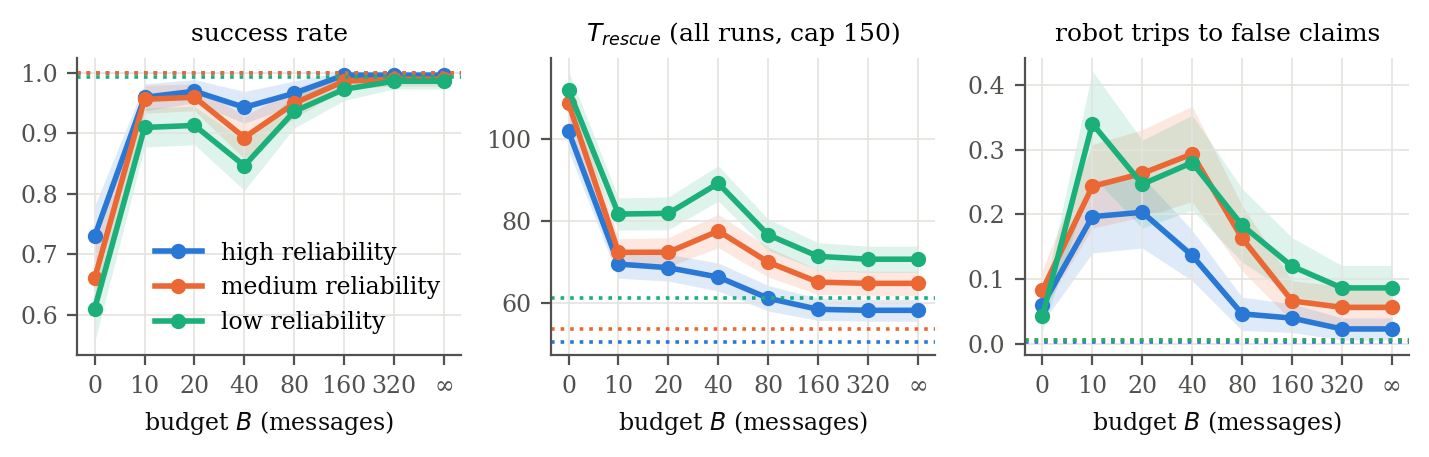
\includegraphics[width=\textwidth]{reliability.png}
\caption{E2: budget sweep (MGM) at three sensor-reliability levels. Dotted lines: centralised reference of the same colour.}
\label{fig:rel}
\end{figure}

\begin{table}[t]
\centering\small
\caption{E2: effect of sensor reliability (MGM). Success rate and $T_{\mathrm{rescue}}$ (all runs, failures counted at
the 150-step limit); last two columns at $B=\infty$.}\label{tab:rel}
\begin{tabular}{@{}lcccc|cccc|cc@{}}
\toprule
 & \multicolumn{4}{c|}{Success} & \multicolumn{4}{c|}{$T_{\mathrm{rescue}}$} & wrong & false \\
Reliab. & Central & $B{=}\infty$ & $B{=}20$ & $B{=}0$ & Central & $B{=}\infty$ & $B{=}20$ & $B{=}0$ & claims & trips \\
\midrule
high & 1.00 & 1.00 & 0.97 & 0.73 & 50.5 & 58.2 & 68.6 & 101.9 & 0.20 & 0.02 \\
medium & 1.00 & 0.99 & 0.96 & 0.66 & 53.6 & 64.8 & 72.4 & 108.8 & 0.56 & 0.06 \\
low & 0.99 & 0.99 & 0.91 & 0.61 & 61.2 & 70.7 & 81.9 & 112.0 & 0.66 & 0.09 \\

\bottomrule
\end{tabular}
\end{table}

\begin{figure}[t]
\centering
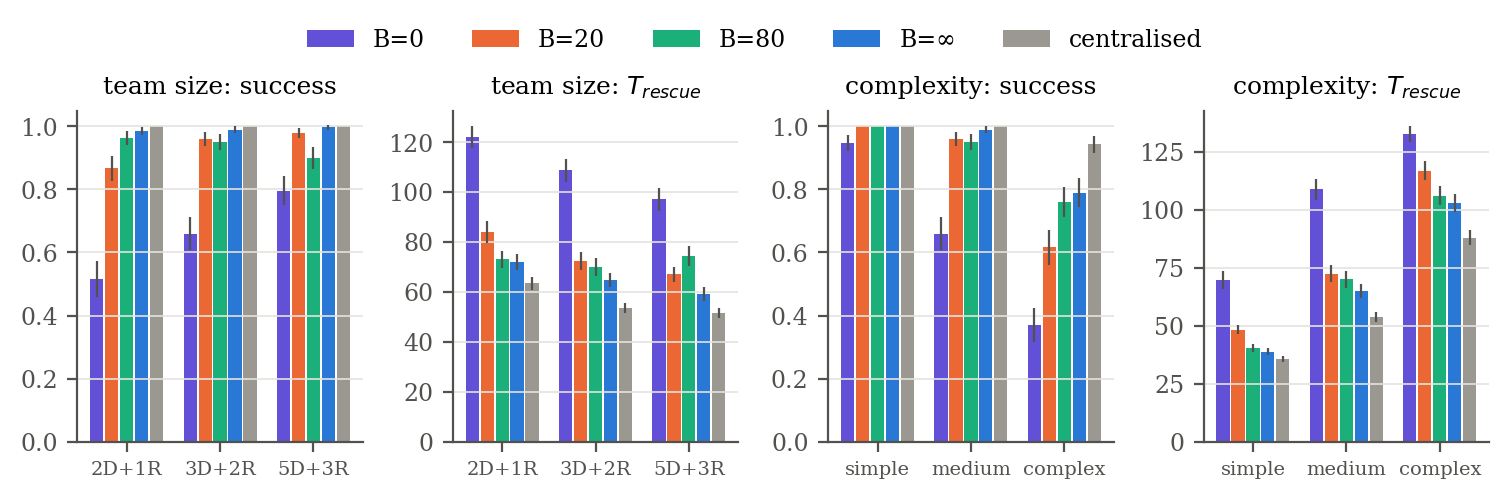
\includegraphics[width=\textwidth]{team_complexity.png}
\caption{E3/E4: success and completion time across team sizes and building complexity at four budgets (MGM) and for the
centralised reference (95\% CIs).}
\label{fig:tc}
\vspace{4pt}
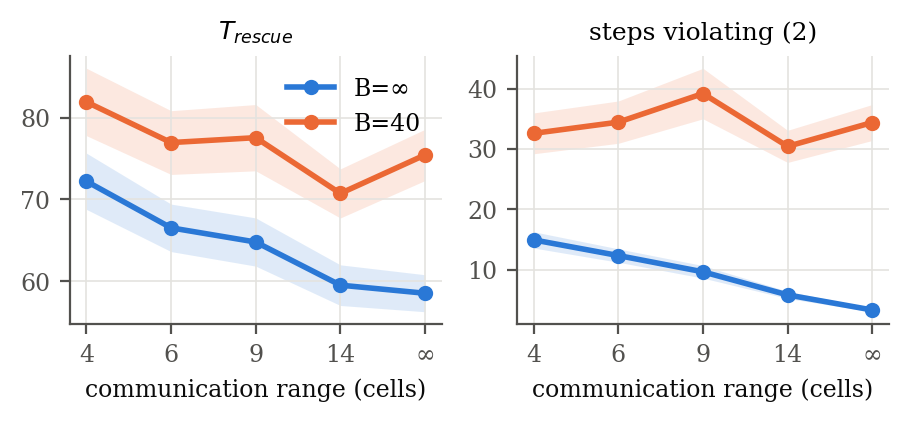
\includegraphics[width=0.55\textwidth]{range.png}
\caption{E5: completion time and constraint-(2) violations against communication range.}\label{fig:range}
\end{figure}

\subsection{E2: is communication more valuable when sensors are noisy?}
Yes (Figure~\ref{fig:rel}, Table~\ref{tab:rel}). The success gap between no communication and unrestricted
communication grows from 0.27 (high reliability) to 0.33 (medium) and 0.38 (low), and the robots' wait for the victim
location without communication grows from 71 to 84 steps. With noisy sensors no single agent can confirm the victim
quickly, so pooling evidence across agents matters more. The review's secondary hypothesis---that sharing also spreads
false alarms---is confirmed in a specific form (right panel of Figure~\ref{fig:rel}): robot trips to empty claimed cells
peak at \emph{small and intermediate} budgets ($B=10$--$40$), where a claim is transmitted but most of the evidence that
would later refute it is not, and they vanish as $B$ grows. Under low reliability this again produces a dip at $B=40$
(success 0.85, vs.\ 0.91 at $B=10$): a little noisy information beyond the victim report can be worse than none.

\subsection{E3--E5: is the trend specific to one team or one map?}
The shape of the curve---large loss at $B=0$, most of it recovered by a small budget---holds for every team size and map
(Figure~\ref{fig:tc}). \textbf{Team size:} the smallest team suffers most without communication (success 0.52 for
2D+1R vs.\ 0.80 for 5D+3R) because a single robot must find the victim alone. The centralised message volume grows
linearly with team size (205$\to$439) while the decentralised volume at $B=\infty$ stays below half of it (88$\to$215).
The largest team also shows the intermediate-budget dip (0.98 at $B=20$, 0.90 at $B=80$), with the most wrong claims
(1.8 per run): more agents sharing partial noisy evidence produce more false claims. \textbf{Complexity:} the gap widens
with the building. On the simple map even $B=0$ succeeds in 95\% of runs; on the complex $28\times28$ map success falls to
0.37 without communication, and the decentralised team stays well below the centralised one even with unrestricted
budget (0.79 vs.\ 0.94), because the fixed 9-cell range covers a smaller fraction of the building and there is more map to
discover. \textbf{Communication range (Figure~\ref{fig:range}):} with $B=\infty$, widening the range steadily closes the
gap ($T=72.2$ at $r_c=4$ to 58.5 with global broadcast vs.\ 53.6 centralised) and removes most duplicated assignments
(15$\to$3 steps); with $B=40$ the budget, not connectivity, dominates (duplicates stay at 30--39 steps for every range).

\begin{figure}[t]
\centering
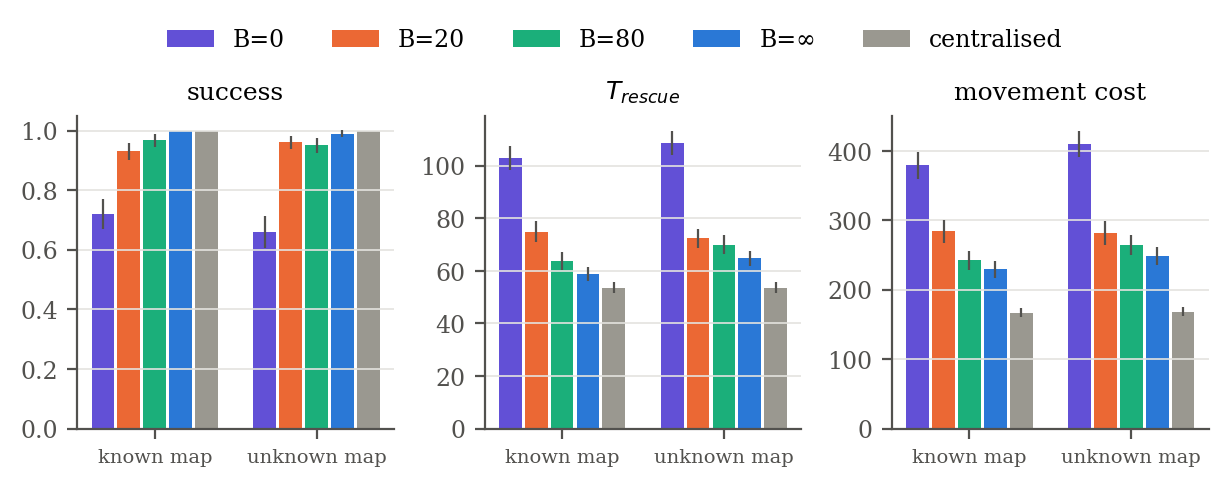
\includegraphics[width=0.66\textwidth]{map_knowledge.png}
\caption{E6: known floor plan vs.\ unknown (discovered) floor plan at four budgets (MGM) and centralised.}
\label{fig:map}
\end{figure}

\subsection{E6: what does not knowing the floor plan cost?}
The centralised coordinator is unaffected by having to discover the map ($T=53.6$ either way): it pools every agent's
terrain observations instantly. The decentralised team is not: with unrestricted budget its completion time rises from
58.8 to 64.8 (gap to centralised 10\%$\to$21\%) and its movement by 8\%; without communication success falls from 0.72 to
0.66 (Figure~\ref{fig:map}). Discovered terrain is therefore a second kind of information---after the victim
report---that the budget must carry. Conversely, at low budgets the unknown map slightly \emph{reduces} false claims (0.59
vs.\ 1.49 at $B=20$), because the wider prior requires more evidence before a claim is made.

\subsection{Discussion and limitations}
The value of communication is concentrated in the few messages that carry the drone-to-robot handoff; without them
complementary agent types are of little use. Further budget buys less redundant exploration, shared terrain and better
coordination. More budget is not always better: at intermediate budgets partial, noisy evidence and coordination messages can do harm,
which suggests that a budget-aware messaging rule---deciding between evidence, terrain and coordination messages---is
the natural next step. Limitations: a single victim; static hazards; independent sensor noise; lossless messages
within range; optimistic planning on unknown cells; MGM and DSA-C reach local optima only; results depend on our cost
weights and are simulation results, not claims about real emergency-response systems.

\section{Contribution}\label{sec:contrib}
All tasks assigned in the project review were completed; each member also contributed to integration, testing,
debugging and writing.
\begin{itemize}\setlength\itemsep{0pt}
\item \textbf{Boinapally Dhanvini} --- literature review (multi-agent SAR, heterogeneous teams, CSP/DCOP) and the formal
model of Section~\ref{sec:formulation}; choice of MGM/DSA-C over ADOPT and derivation of the task set and cost functions
from~\eqref{eq:obj}. \emph{Status: fulfilled.}
\item \textbf{Bollineni Snehitha Rao} --- environment and agent modelling: building generation, obstacles, hazards,
movement, the observation model~\eqref{eq:obs} and reliability/complexity settings. She also built an independent
prototype whose two key ideas---a floor plan discovered by sensing and DSA-C allocation---were integrated into the final
code (\texttt{sar/mapknow.py}, DSA-C in \texttt{sar/sim.py}). \emph{Status: fulfilled.}
\item \textbf{Jils Shah} --- centralised Hungarian baseline and decentralised MGM/DSA-C coordination
(\texttt{sar/allocation.py}, \texttt{sar/sim.py}); communication budget, messaging rule and identical message accounting
for all methods; integration of the final simulator; unit tests checking constraints \eqref{eq:c2}--\eqref{eq:c4}, the
budget and the optimality of the baseline. \emph{Status: fulfilled.}
\item \textbf{Thaker Shivangi Pareshkumar} --- experimental design and analysis (\texttt{experiments/}): the six
experiments with matched seeds, metrics, plots and tables, and the interpretation in Section~\ref{sec:results}.
\emph{Status: fulfilled.}
\end{itemize}

\section{Conclusion}
We built a simulator of heterogeneous search and rescue in a building whose layout and victim location are unknown,
under a communication budget, and compared an exact centralised task allocation with decentralised MGM and DSA-C over
30{,}600 matched episodes. Performance falls sharply only when communication is (almost) removed: two messages per
agent, used for the drone-to-robot handoff, recover 90\% of the lost success, and an unrestricted decentralised team
nearly matches the centralised success rate with 48\% of its messages, at a 21\% time cost of which half is due to discovering
the map. Communication matters more when sensors are noisy, for smaller teams and in larger buildings; at small budgets
observation sharing should take priority over coordination messages, and DSA-C is the more message-efficient
coordinator. Code, data, figures and instructions to reproduce every number are in the repository.

\footnotesize
\begin{thebibliography}{9}\setlength\itemsep{0pt}
\bibitem{queralta2020} J.~Pe\~na Queralta, J.~Taipalmaa, B.~Can Pullinen, V.~K. Sarker, T.~Nguyen Gia, H.~Tenhunen, M.~Gabbouj, J.~Raitoharju, and T.~Westerlund. Collaborative multi-robot search and rescue: Planning, coordination, perception, and active vision. \emph{IEEE Access}, 8:191617--191643, 2020.
\bibitem{fioretto2018} F.~Fioretto, E.~Pontelli, and W.~Yeoh. Distributed constraint optimization problems and applications: A survey. \emph{Journal of Artificial Intelligence Research}, 61:623--698, 2018.
\bibitem{gunn2015} T.~Gunn and J.~Anderson. Dynamic heterogeneous team formation for robotic urban search and rescue. \emph{Journal of Computer and System Sciences}, 81(3):553--567, 2015.
\bibitem{korsah2013} G.~A. Korsah, A.~Stentz, and M.~B. Dias. A comprehensive taxonomy for multi-robot task allocation. \emph{The International Journal of Robotics Research}, 32(12):1495--1512, 2013.
\bibitem{modi2005} P.~J. Modi, W.-M. Shen, M.~Tambe, and M.~Yokoo. ADOPT: Asynchronous distributed constraint optimization with quality guarantees. \emph{Artificial Intelligence}, 161(1--2):149--180, 2005.
\bibitem{burgard2005} W.~Burgard, M.~Moors, C.~Stachniss, and F.~E. Schneider. Coordinated multi-robot exploration. \emph{IEEE Transactions on Robotics}, 21(3):376--386, 2005.
\bibitem{maheswaran2004} R.~T. Maheswaran, J.~P. Pearce, and M.~Tambe. Distributed algorithms for DCOP: A graphical-game-based approach. In \emph{Proc.\ ISCA PDCS}, pages 432--439, 2004.
\bibitem{zhang2005} W.~Zhang, G.~Wang, Z.~Xing, and L.~Wittenburg. Distributed stochastic search and distributed breakout: properties, comparison and applications to constraint optimization problems in sensor networks. \emph{Artificial Intelligence}, 161(1--2):55--87, 2005.
\bibitem{kuhn1955} H.~W. Kuhn. The Hungarian method for the assignment problem. \emph{Naval Research Logistics Quarterly}, 2(1--2):83--97, 1955.
\end{thebibliography}

\end{document}
